%	This LaTeX file is written by Zhiyang Ong as a template for creating presentation slides.

%	The MIT License (MIT)

%	Copyright (c) <2015> <Zhiyang Ong>

%	Permission is hereby granted, free of charge, to any person obtaining a copy of this software and associated documentation files (the "Software"), to deal in the Software without restriction, including without limitation the rights to use, copy, modify, merge, publish, distribute, sublicense, and/or sell copies of the Software, and to permit persons to whom the Software is furnished to do so, subject to the following conditions:

%	The above copyright notice and this permission notice shall be included in all copies or substantial portions of the Software.

%	THE SOFTWARE IS PROVIDED "AS IS", WITHOUT WARRANTY OF ANY KIND, EXPRESS OR IMPLIED, INCLUDING BUT NOT LIMITED TO THE WARRANTIES OF MERCHANTABILITY, FITNESS FOR A PARTICULAR PURPOSE AND NONINFRINGEMENT. IN NO EVENT SHALL THE AUTHORS OR COPYRIGHT HOLDERS BE LIABLE FOR ANY CLAIM, DAMAGES OR OTHER LIABILITY, WHETHER IN AN ACTION OF CONTRACT, TORT OR OTHERWISE, ARISING FROM, OUT OF OR IN CONNECTION WITH THE SOFTWARE OR THE USE OR OTHER DEALINGS IN THE SOFTWARE.

%	Email address: echo "cukj -wb- 23wU4X5M589 TROJANS cqkH wiuz2y 0f Mw Stanford" | awk '{ sub("23wU4X5M589","F.d_c_b. ") sub("Stanford","d0mA1n"); print $5, $2, $8; for (i=1; i<=1; i++) print "6\b"; print $9, $7, $6 }' | sed y/kqcbuHwM62z/gnotrzadqmC/ | tr 'q' ' ' | tr -d [:cntrl:] | tr -d 'ir' | tr y "\n"



%%%%%%%%%%%%%%%%%%%%%%%%%%%%%%%%%%%%%%%%%%%%%%
%	Preamble

%	Acknowledgement:
%		This is based on a template provided to me by Dott. Francesco Stefanni, from the University of Verona in January 2011.
%
%	Number the slides per section. This makes it easier to track the index of the slides (or number of slides) per section, as opposed to the cumulative number of slides. When I manually track the number of slides for a presentation, each time I refactor the set of slides, I would have to update the slide numbers. I want the computer to do this automatically. Hence, I shall not do this manually.



%	Use the Beamer package to create the presentation slides.
\documentclass[xcolor={usenames,dvipsnames},hyperref={hyperindex,bookmarks}]{beamer}


%%%%%%%%%%%%%%%%%%%%%%%%%%%%%%%%%%%%%%%%%%%%%%
%	Import and Customize LaTeX packages.
\usepackage{beamerthemesplit}


%	Package for typesetting the following symbol: $\mathfrak{S}$
%\usepackage{amssymb}

%\mode<presentation>
%{ \usetheme{boxes} }

%	Select the presentation mode.
\mode<presentation>{
	\usetheme[logos=true,pagenumbers=true,background=true]{Esd}
}
\setbeamercovered{transparent}
%\setbeamercovered{invisible}


%	Import package to facilitate typesetting of algorithms.
\usepackage{listings}

\lstset{
  language=C++,
  tabsize=4,
%  basicstyle=\ttfamily\color{black}\small,
  basicstyle=\ttfamily\color{black},
%  backgroundcolor=\color{lightgray},
%  backgroundcolor=\color{white},
  keywordstyle=\color{Purple}\bfseries,
  identifierstyle=\color{OliveGreen},
  commentstyle=\color{Gray}\itshape,
  stringstyle=\color{CarnationPink},
  showstringspaces=false,
  showtabs=false,
  showspaces=false
}


\definecolor{lightgray}{gray}{0.95}
\font\emailtt=cmtt9

%	Set up configuration for hyperlinks.
%\usepackage[pdftex]{hyperref}	-- Option clash
\hypersetup{
    pdftitle={Programming Style for C},     % title
    pdfauthor={Francesco Stefanni},                 % author
    pdfsubject={A programming style for C}, % subject of the document
    pdfcreator={Creator},                           % creator of the document
    pdfproducer={dvipdft},                          % producer of the document
% Modified by Zhiyang Ong on Feb 7, 2011 to improve the way hyperlinks are colored in these presentation slides
	pdfkeywords={LaTeX, graphics, color},
%    pdfkeywords={C, C++, programming style},        % list of keywords
%
%    bookmarks=true,         % show bookmarks bar?
    unicode=false,          % non-Latin characters in Acrobats bookmarks
    pdftoolbar=true,        % show Acrobats toolbar?
    pdfmenubar=true,        % show Acrobats menu?
    pdffitwindow=false,     % window fit to page when opened
% Modified by Zhiyang Ong on Feb 7, 2011 to improve the way hyperlinks are colored in these presentation slides
	pdfpagemode=UseOutlines,bookmarks, bookmarksopen,
	pdfstartview=FitH, colorlinks, linkcolor=blue, citecolor=blue, urlcolor=red,
%    pdfstartview={Fit},    % fits the width of the page to the window
    pdfnewwindow=true,      % links in new window
% Modified by Zhiyang Ong on Feb 7, 2011 to improve the way hyperlinks are colored in these presentation slides
	colorlinks=red,        % false: boxed links; true: colored links
	linkcolor=red,          % color of internal links
%    colorlinks=false,        % false: boxed links; true: colored links
%    linkcolor=red,          % color of internal links
    citecolor=green,        % color of links to bibliography
    filecolor=magenta,      % color of file links
    urlcolor=red,           % color of external links
    pdfpagemode=FullScreen
    %
    %pdfpagelabels=false
}

%\usepackage[all]{hypcap}




%%%%%%%%%%%%%%%%%%%%%%%%%%%%%%%%%%%%%%%%%%%%%%
%	Added by Zhiyang Ong on Feb 7, 2011 to allow figures to be places side-by-side
%\usepackage{subfigure}









%%%%%%%%%%%%%%%%%%%%%%%%%%%%%%%%%%%%%%%%%%%%%%
%%%%%%%%%%%%%%%%%%%%%%%%%%%%%%%%%%%%%%%%%%%%%%
%%%%%%%%%%%%%%%%%%%%%%%%%%%%%%%%%%%%%%%%%%%%%%
%%%%%%%%%%%%%%%%%%%%%%%%%%%%%%%%%%%%%%%%%%%%%%
%%%%%%%%%%%%%%%%%%%%%%%%%%%%%%%%%%%%%%%%%%%%%%
%%%%%%%%%%%%%%%%%%%%%%%%%%%%%%%%%%%%%%%%%%%%%%
%%%%%%%%%%%%%%%%%%%%%%%%%%%%%%%%%%%%%%%%%%%%%%


%	Quantum Model Checking Is Not Evil: It Is Mandatory For Quantum Robots


%	First slide of the presentation
\title[Quantum Reachability Analysis]
{\huge 
%Optimization and Taint Analysis of Microarchitecture Synthesis Software}
Taint Analysis of Microarchitecture Synthesis Software}
\subtitle{Not Using It to Secure Microarchitectures is Foolish}
\author{Zhiyang Ong}
\institute{
	Department of Electrical and Computer Engineering \\
	Dwight Look College of Engineering,\\
	Texas A\&M University \\
	College Station, TX
}
\date{\today}	% (optional)
\subject{Subject Title}

%	This set of presentation slides is based on \cite{Ying2014a}, from my BibTeX research database.







%%%%%%%%%%%%%%%%%%%%%%%%%%%%%%%%%%%%%%%%%%%%%%
%	Do nothing in this section of the LaTeX document

\begin{document}

\begin{frame}
\titlepage
\end{frame}



%	Table of Contents
%	\AtBeginSection[]		% Do nothing for \subsection*
%	{
%		\begin{frame}
%	%		\frametitle{\textcolor{yellow}{Table of Contents}}
%			\frametitle{Table of Contents}
%	%		\textcolor{yellow}{\tableofcontents[currentsection]}
%			\tableofcontents[currentsection,currentsubsection]
%		\end{frame}
%	}
%	
%	\AtBeginSubsection[]		% Do nothing for \subsection*
%	{
%	\begin{frame}
%	\tableofcontents[currentsection,currentsubsection]
%	\end{frame}
%	}

%	\section*{Outline}
%	\begin{frame}
%	\tableofcontents
%	\end{frame}



%%%%%%%%%%%%%%%%%%%%%%%%%%%%%%%%%%%%%%%%%%%%%%
%
%	Slides begin HERE!!!
%
%%%%%%%%%%%%%%%%%%%%%%%%%%%%%%%%%%%%%%%%%%%%%%


%%%%%%%%%%%%%%%%%%%%%%%%%%%%%%%%%%%%%%%%%%%%%%
%	Preamble

%	Slide #1
%\section{Introduction}
\begin{frame}
	\frametitle{Background}
	Microarchitecture synthesis software is used to generate cycle-accurate/RTL designs of microarchitectures. \\
	\ \\
	Taint analysis has been used to determine security loopholes of software. \\
	\ \\
	Project Goal: Apply taint analysis to determine the security loopholes of the microarchitecture synthesis software.
\end{frame}




%	Slide #2
\frame
{
	\frametitle{Timeline of Milestones}

	\begin{itemize}
	\item Benchmarks (now): %\vspace{-0.2cm}
		\begin{enumerate} %\itemsep -2pt
		\item Rocket chip: https://github.com/ucb-bar/rocket-chip
		\item OpenSoCFabric: https://github.com/ucb-bar/OpenSoCFabric
		\item chisel-torture: https://github.com/ucb-bar/chisel-torture
		\end{enumerate}
	\item Instruction set architecture: RISC-V ISA
	\item Learning Chisel: Early October
	\item firrtl parser: Mid October
	\item Taint analysis: %\vspace{-0.2cm}
		\begin{enumerate} %\itemsep -2pt
		\item Late October - Early November
		\item Multi-cycle processor's control logic 
		\item Pipelined processor's control logic 
		\item Branch prediction FSM
		\item Cache coherence FSM
		\end{enumerate}
	%\item System-level Design for Testability (DFT) Synthesis: Late November
	\item Design for Testability (DFT) Synthesis: Late November
	\item More taint analysis on DFT components: Late November
%	\item introduce the notion of reachability analysis, from classical/traditional formal verification, before reachability analysis is introduced for formally verifying quantum systems, including quantum robots.
	\item Regression testing: Early December
	\end{itemize}
}





%	Slide #3
%\section{Pictures}
\begin{frame}
	\frametitle{Pictures}

%	branch-prediction
%	cache-coherence
%	multi-cycle-processor-fsm-ctrl-logic	
	\begin{figure}[h]
	\centering 
	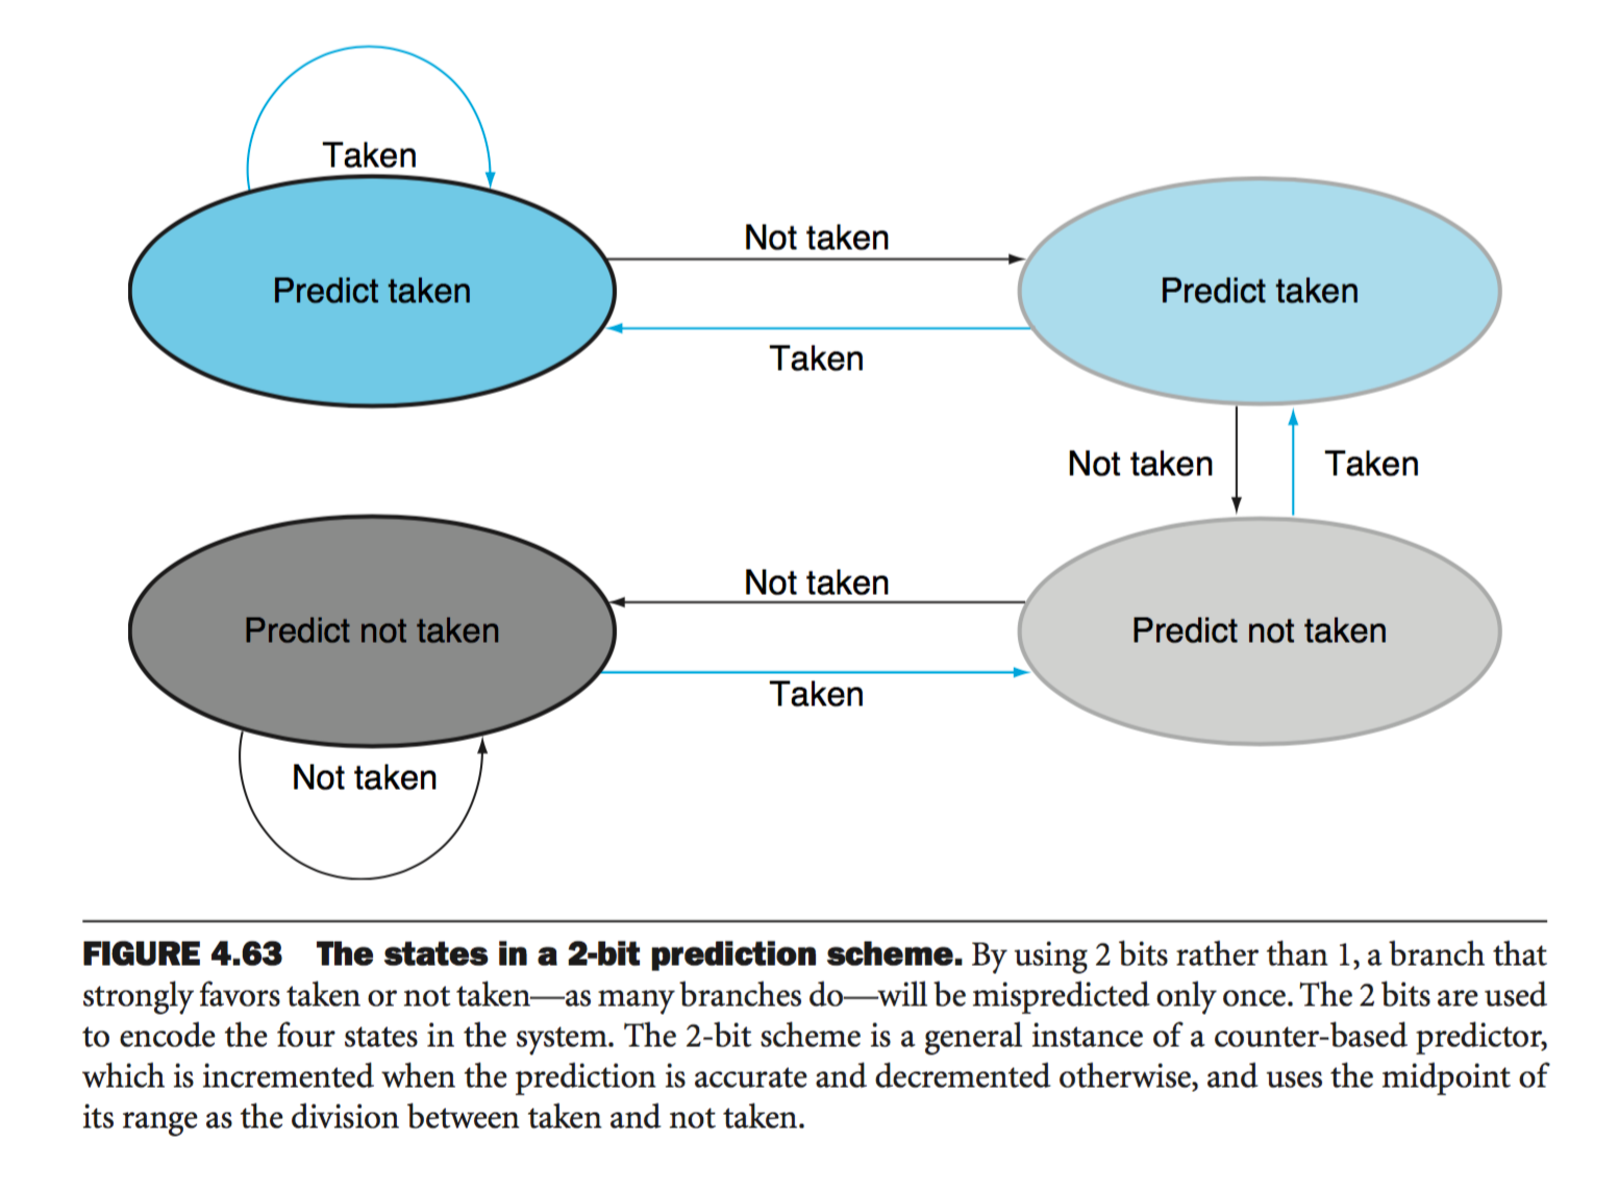
\includegraphics[height=2.2in]{./pics/branch-prediction}
	\caption{Branch prediction FSM}
	\label{fig:branchprediction}
	\end{figure}
	
\end{frame}


%	Slide #4
%\section{Pictures}
\begin{frame}
	\frametitle{Pictures}

%	branch-prediction
%	cache-coherence
%	multi-cycle-processor-fsm-ctrl-logic	
	\begin{figure}[h]
	\centering 
	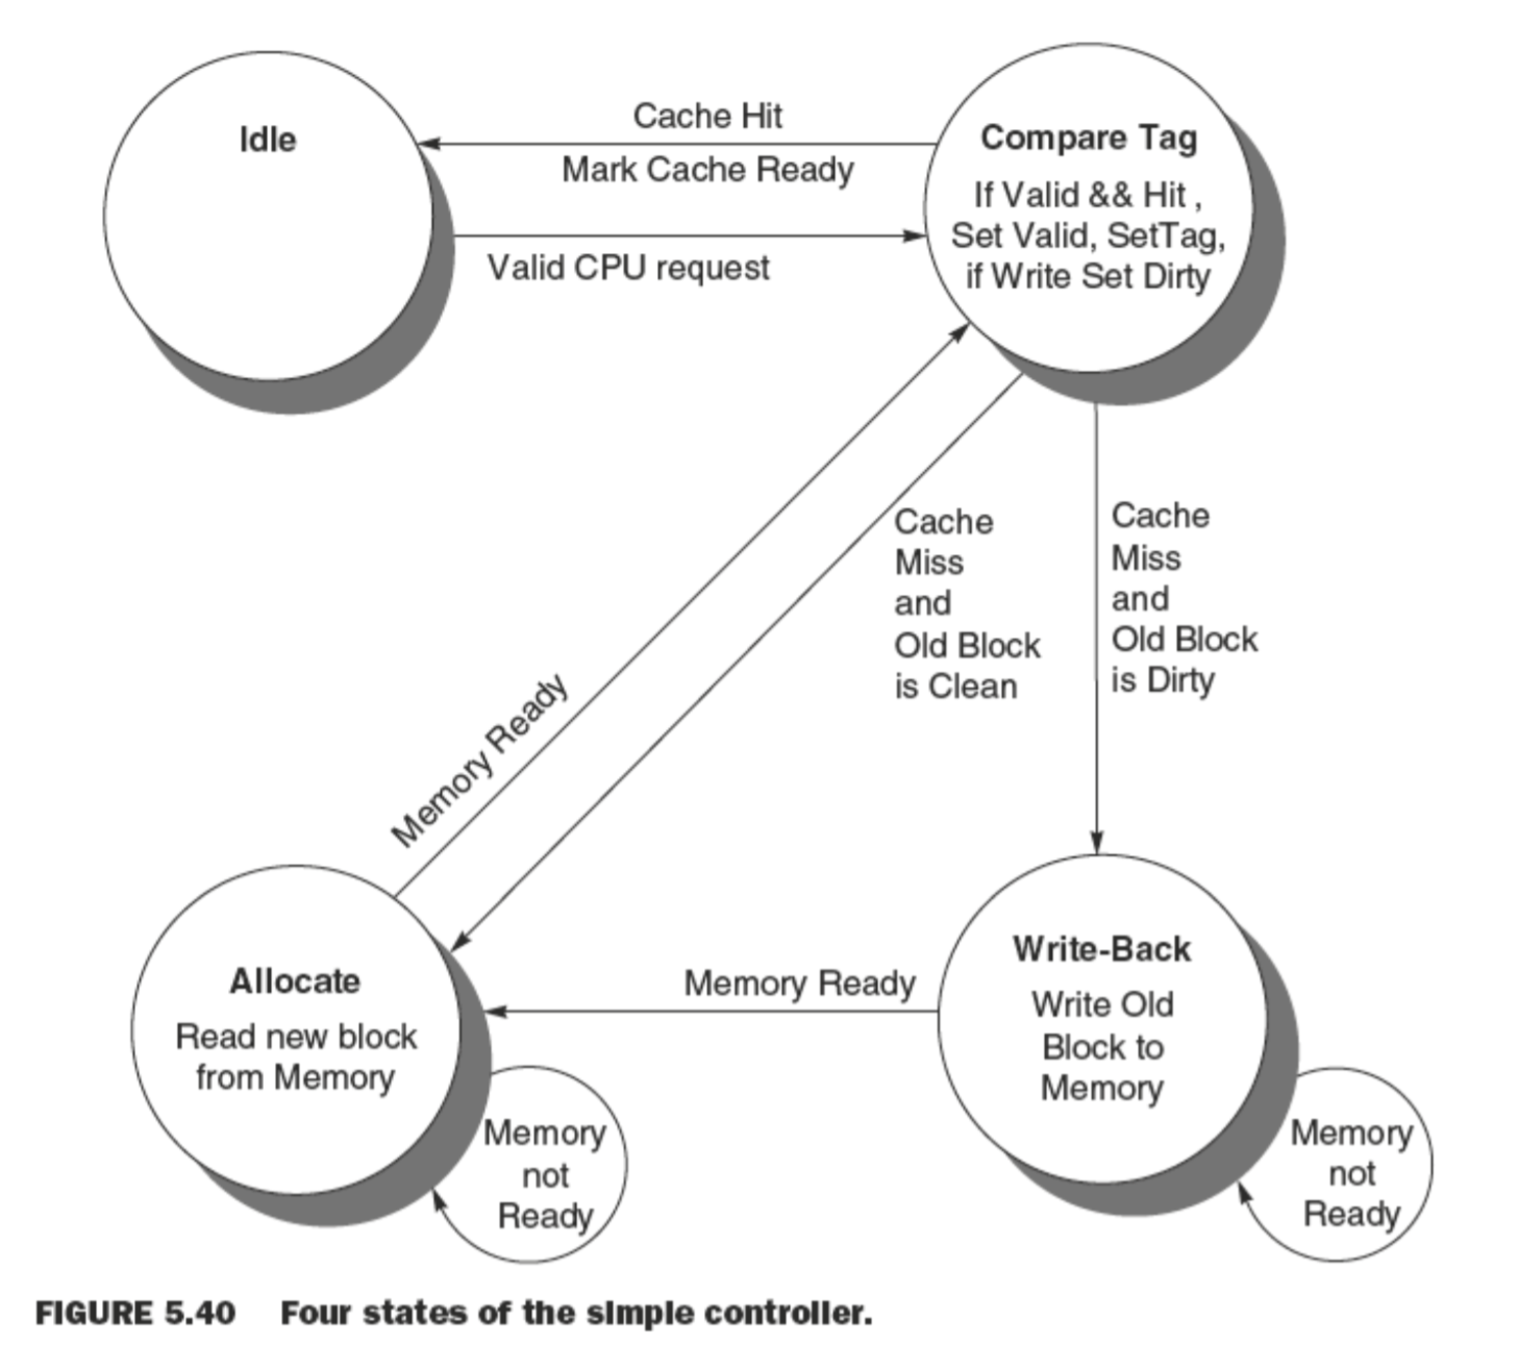
\includegraphics[height=2.2in]{./pics/cache-coherence}
	\caption{Cache coherence FSM}
	\label{fig:cachecoherence}
	\end{figure}

\end{frame}







%	Slide #5
%\section{Pictures}
\begin{frame}
	\frametitle{Pictures}

%	branch-prediction
%	cache-coherence
%	multi-cycle-processor-fsm-ctrl-logic	
	\begin{figure}[h]
	\centering 
	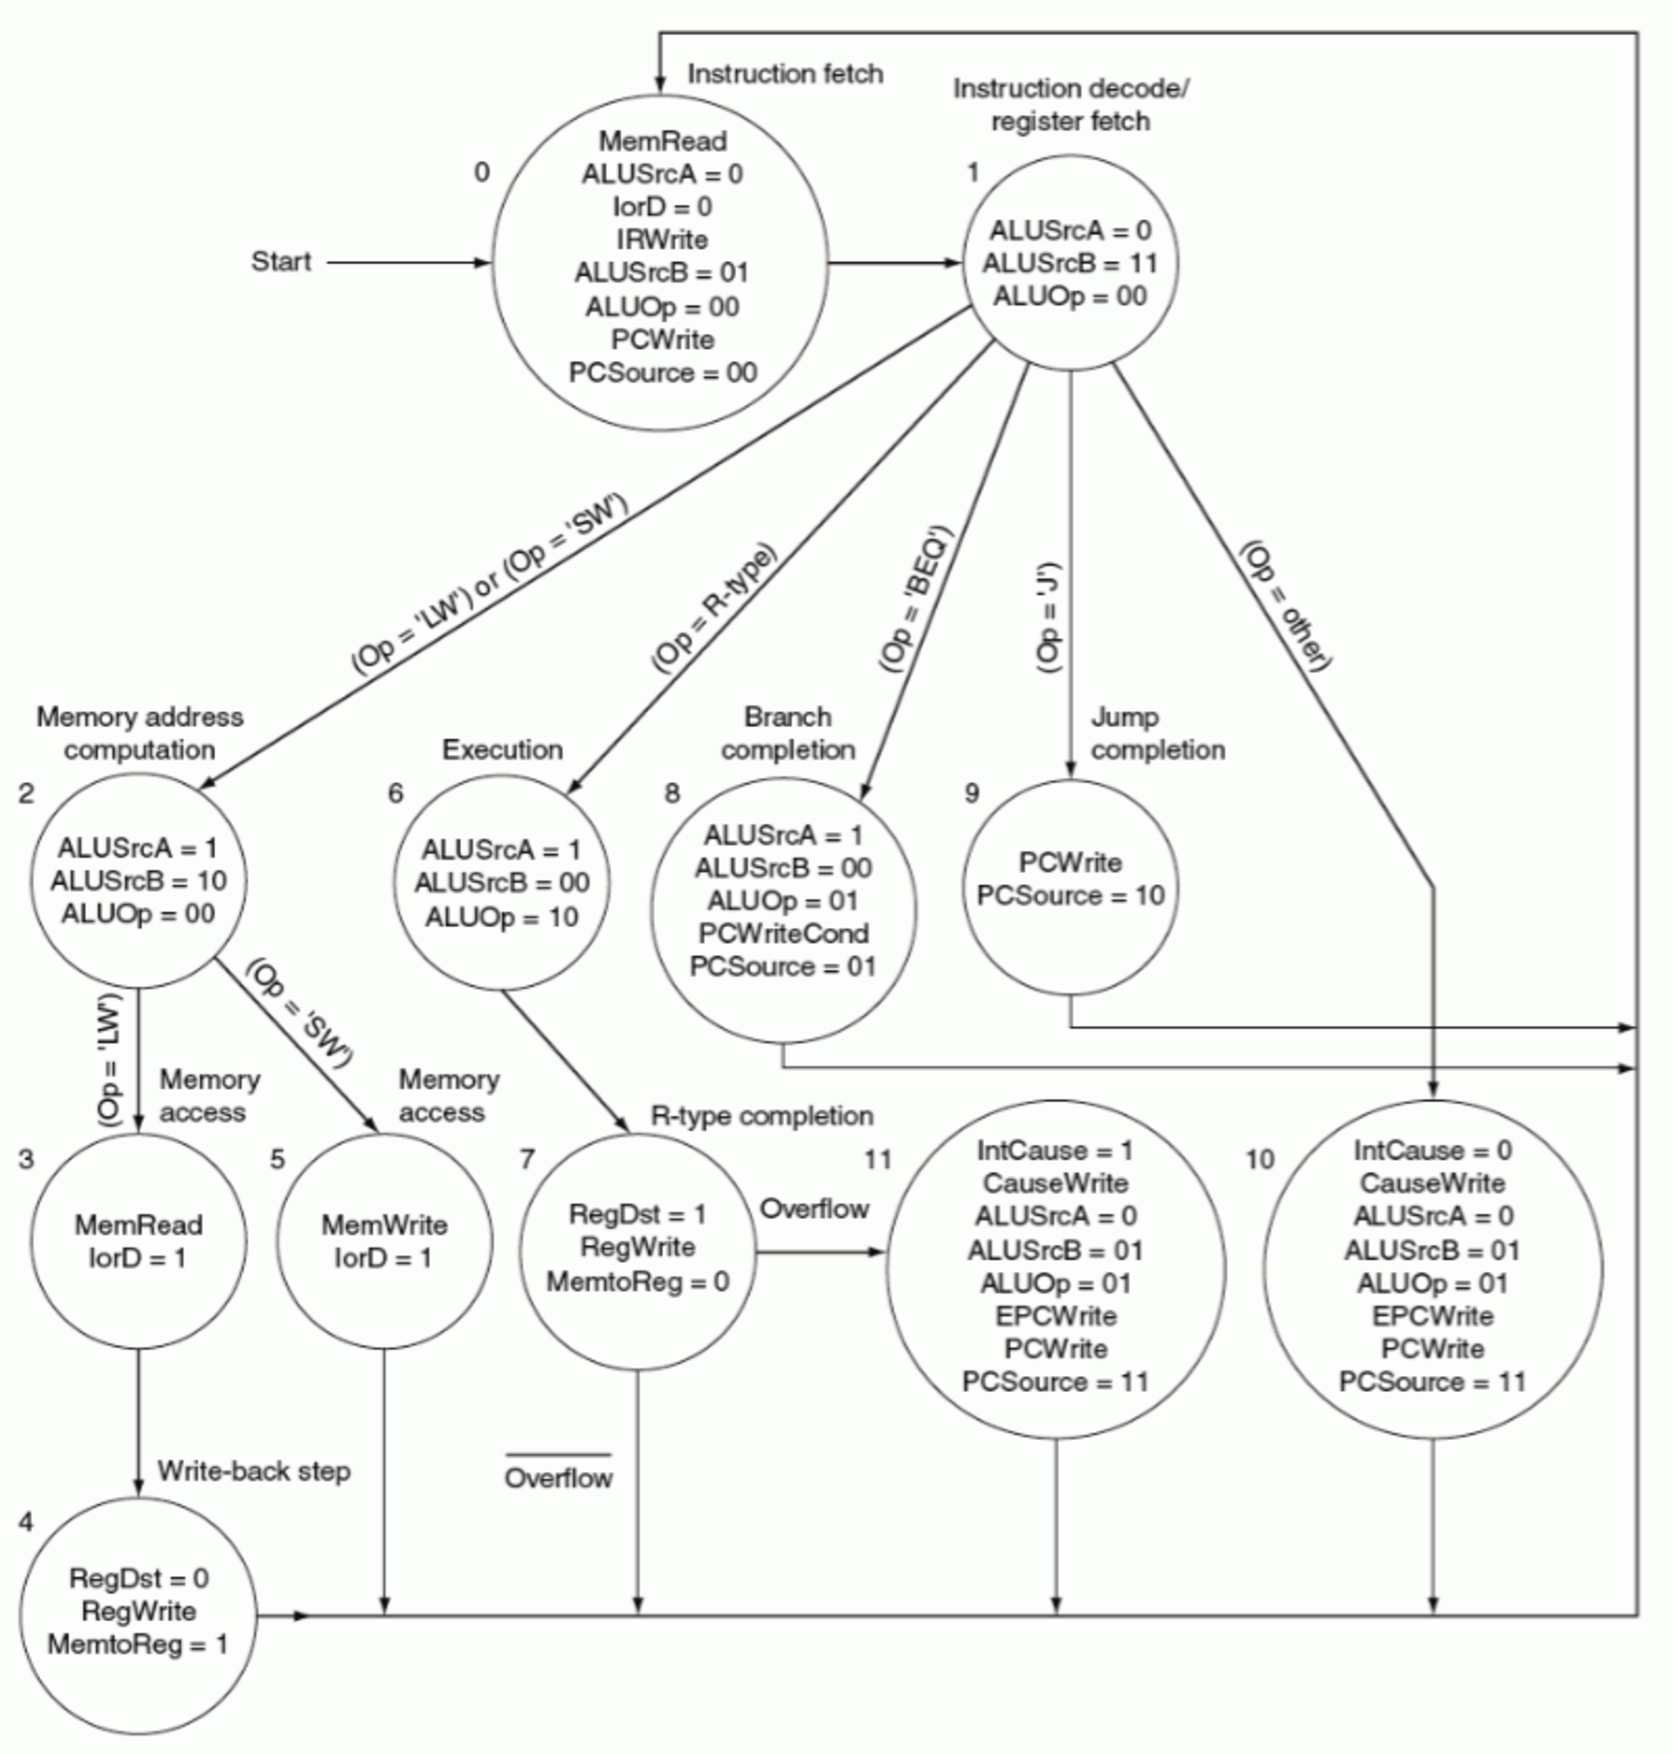
\includegraphics[height=2.2in]{./pics/multi-cycle-processor-fsm-ctrl-logic}
	\caption{FSM of multi-cycle processor's control logic}
	\label{fig:multicycleprocessorfsmctrllogic}
	\end{figure}
\end{frame}









%%%%%%%%%%%%%%%%%%%%%%%%%%%%%%%%%%%%%%%%%%%%%%

%\section{Background Information}

%\subsection{Background Information}
%
%\frame
%{
%	\frametitle{Coursework Related to Electronic Design Automation}
%
%	\begin{itemize}
%	\item<1-> University of Southern California: \vspace{-0.05cm}
%		\begin{itemize} \itemsep -1pt
%		\item Electronic Design Automation + Digital VLSI Testing: \vspace{-0.1cm}
%			\begin{itemize} \itemsep -1pt
%			\item EE 680 -- Computer Aided Design of Digital Systems I
%			\item EE 599/581 -- Mathematical Foundations for Computer Aided Design of VLSI Systems
%			\item EE 658 -- Diagnosis and Design of Reliable Digital Systems
%			\end{itemize}
%		\item Digital VLSI Design: \vspace{-0.1cm}
%			\begin{itemize} \itemsep -1pt
%			\item EE 477L -- MOS VLSI Circuit Design
%			\item EE 577A/B -- VLSI System Design
%			\end{itemize}
%		\end{itemize}
%	\item<2-> University of Adelaide: \vspace{-0.05cm}
%		\begin{itemize} \itemsep -1pt
%		\item Introductory Digital VLSI Design: \vspace{-0.1cm}
%			\begin{itemize} \itemsep -1pt
%			\item Elec Eng 4037 -- Digital Microelectronics
%			\item Elec Eng 3017 -- Digital Electronics
%			\end{itemize}
%		\item Software Engineering: \vspace{-0.1cm}
%			\begin{itemize} \itemsep -1pt
%			\item Comp Sci 3006 -- Software Engineering and Project
%			\end{itemize}
%		\item Relevant classes for my research topic: \vspace{-0.1cm}
%			\begin{itemize} \itemsep -1pt
%			%\item Elec Eng 4044 -- RF Engineering IV
%			%\item Elec Eng 3021 -- Electrical Energy Systems
%			%\item Elec Eng 4042 -- Power Electronics and Drive Systems
%			\item Elec Eng 3015 -- Communications, Signals, \& Systems
%			\item Elec Eng 3016 -- Control III
%			\item Elec Eng 3018 -- RF Engineering III
%			%\item Elec Eng 3020 -- Embedded Computer Systems
%			\end{itemize}
%		\end{itemize}
%	\end{itemize}
%}









%%%%%%%%%%%%%%%%%%%%%%%%%%%%%%%%%%%%%%%%%%%%%%

%\section{Research and Project Experience}
%
%\subsection{Problem Description}
%
%\frame
%{
%	\frametitle{Research Background}
%
%	\begin{itemize}
%	\item<1-> Literature Review: \vspace{-0.05cm}
%		\begin{itemize} \itemsep -1pt
%		\item Robotic Surgery + Biomedical MEMS
%		\end{itemize}
%	\item<2-> Honors research project / Senior thesis: \vspace{-0.05cm}
%		\begin{itemize} \itemsep -1pt
%		\item Complex Systems + Evolutionary Computation
%		\end{itemize}
%	\item<3-> Masters Research Project: \vspace{-0.05cm}
%		\begin{itemize} \itemsep -1pt
%		\item Automatic Test Pattern Generation at Electronic System-Level�(Attempted)
%		\item Computer System Performance Analysis (vertical profiling)
%		\end{itemize}
%	\end{itemize}
%}


%%%%%%%%%%%%%%%%%%%%%%%%%%%%%%%%%%%%%%%%%%%%%%

%\section{Research and Project Experience}

%\subsection{Project Experience}
%
%\frame
%{
%	\frametitle{Project Experience}
%
%	\begin{itemize}
%	\item<1-> EDA Software Development: \vspace{-0.05cm}
%		\begin{itemize} \itemsep -1pt
%		\item ATPG for FPGA test generation system
%		\item C++ Parser for IEEE STIL format
%		\item Gate-level logic simulator for combinational VLSI circuits
%		\item Software for crosstalk-aware gate sizing in VLSI circuits
%		\end{itemize}
%	\item<2-> Digital VLSI Design: \vspace{-0.05cm}
%		\begin{itemize} \itemsep -1pt
%		\item Viterbi decoder
%		\item 32-kbit synchronous SRAM with 32-bit words
%		\item 64-bit Ladner-Fischer tree adder
%		\item 32-bit variable length carry-increment adder
%		\end{itemize}
%	\item<3-> Processor Design: \vspace{-0.05cm}
%		\begin{itemize} \itemsep -1pt
%		\item 4-stage pipelined Troy Wideword Processor (128-bit datapath)
%		\item 32-bit MIPS processor (multi-cycle \& pipeline implementations)
%		\item AMD Am2901 microprocessor
%		\end{itemize}
%	\end{itemize}
%}








%%%%%%%%%%%%%%%%%%%%%%%%%%%%%%%%%%%%%%%%%%%%%%








%%%%%%%%%%%%%%%%%%%%%%%%%%%%%%%%%%%%%%%%%%%%%%




%%%%%%%%%%%%%%%%%%%%%%%%%%%%%%%%%%%%%%%%%%%%%%







%%%%%%%%%%%%%%%%%%%%%%%%%%%%%%%%%%%%%%%%%%%%%%
%\section{References}
%
%\frame
%{
%	\frametitle{References}
%
%%	\begin{itemize}
%%	\item \cite{Weng2011}
%%	\end{itemize}
%%}
%
%
%	{\linespread{1}
%	%\bibliographystyle{IEEEtran}
%	\bibliographystyle{plain}
%	%\bibliography{./others/references}
%	%\bibliography{/data/others/notes/references}
%	\bibliography{/data/research/antipastobibtex/references}
%	%\addcontentsline{toc}{chapter}{Bibliography}
%	}
%}

\end{document}


%
%	Trying to delay the not-uncommon path of engineering Ph.D.s who end up becoming "PowerPoint engineers"... Hopefully, slapping together a bunch of presentation slides to talk about any topic in any reasonable finite amount of time is not the most useful skill that I would learn as a grad student... Hey, at least I did it in LaTeX/Beamer!!!






 